\documentclass[]{scrartcl}

\setlength{\parindent}{0em}

%\usepackage[ngerman]{babel}
\usepackage[utf8]{inputenc}
\usepackage{csquotes}
\usepackage[OT2,T1]{fontenc}
\usepackage{amsthm}
\usepackage{amsmath}
\usepackage{amssymb}
\usepackage{mathtools}
\usepackage{nicefrac}
\usepackage{extarrows}
\usepackage[Algorithmus]{algorithm}
\usepackage{algpseudocode}
\usepackage{caption}
\usepackage{subcaption}
\usepackage{tikz}
\usepackage{pgfplots}
\usepackage{graphicx}
\usepackage{color}
\usepackage{enumitem}
\usepackage{hyperref}
\usepackage[ngerman]{babel}
\usepackage{array}
\usepackage{marvosym}
\usepackage{tabularx}
\usepackage{booktabs}

%Easier abs und norm
\DeclarePairedDelimiter\abs{\lvert}{\rvert}%
\DeclarePairedDelimiter\norm{\lVert}{\rVert}%
%
\makeatletter
\let\oldabs\abs
\def\abs{\@ifstar{\oldabs}{\oldabs*}}
%
\let\oldnorm\norm
\def\norm{\@ifstar{\oldnorm}{\oldnorm*}}
\makeatother

\usepackage[
	backend=biber,
	style=alphabetic,
	sorting=ynt,
]{biblatex}
\addbibresource{papers.bib}

\pgfplotsset{compat=1.16}


\DeclareMathOperator{\rank}{rank}
\DeclareMathOperator{\trace}{trace}

\newcommand{\R}{\mathbf{R}}
\newcommand{\newlinenice}{\newline \hspace*{5mm}}
\newcommand{\HRule}[1]{\rule{\linewidth}{#1}}
\newcommand{\hmu}{\hat{\mu}}
\newcommand{\hSig}{\hat{\Sigma}}
\newcommand{\bSig}{\bar{\Sigma}}
\newcommand{\tSig}{\tilde{\Sigma}}
\newcommand{\hSharpe}{\hat{\theta}^2}

%\theoremstyle{plain}
%\newtheorem{hlem}{Hilfslemma}
\newtheorem{satz}{Satz}[section]
\newtheorem{theorem}[satz]{Theorem}
\newtheorem{lemma}[satz]{Lemma}
\newtheorem{kor}[satz]{Corollary}
%\theoremstyle{definition}
\newtheorem{defi}[satz]{Definition}
%\theoremstyle{remark}
\newtheorem{rem}[satz]{Remark}
\newtheorem{exa}[satz]{Example}



\begin{document}
	\begin{titlepage} % Suppresses displaying the page number on the title page and the subsequent page counts as page 1
	
	\raggedleft % Right align the title page
	
	\rule{1pt}{0.98\textheight} % Vertical line
	\hspace{0.05\textwidth} % Whitespace between the vertical line and title page text
	\parbox[b]{0.9\textwidth}{ % Paragraph box for holding the title page text, adjust the width to move the title page left or right on the page
		
		{\Huge\bfseries Implementierung eines\\[0.1\baselineskip]
		Neuroevolutionsalgorithmus zur\\[0.1\baselineskip]
		Optimierung von Topologie und Hyperparametern eines \\[0.1\baselineskip]
		künstlichen neuronalen Netzes} \\[0\baselineskip] % Titel
		
		{\Large Ein genetischer Algorithmus zur Automatiserung\\[0.2\baselineskip] von Trainingsprozessen. }\\[2.2\baselineskip] % Untertitel
		
		\vspace{0.1\textheight}

		{\huge Fachpraktikumsbericht}\\[2.4\baselineskip] % Subtitle

		{von \Large\textsc{justus will}}\\[2.4\baselineskip]
		
		\vspace{0.3\textheight}
		
		{\Large \today}
	}
	
\end{titlepage}

%This title page was originally created by Peter Wilson but has been extensively modified for 'https://www.latextemplates.com/template/vertical-line-title-page' by Vel.
	\thispagestyle{empty}
	\pagestyle{empty}
	\newpage
	\tableofcontents
	\newpage
	\pagestyle{plain}
	

\section{Einleitung}

	Der größer werdende Einfluss von künstlicher Intelligenz und machinellem Lernen ist in unserer Gesellschaft nicht mehr zu leugnen.
	In vielen Bereichen haben sich sogenannte künstliche neuronale Netzwerke als vielseitiges Mittel zur Findung von Mustern und Lösung von Problemen erwiesen.
	Unter anderem in Spracherkennung, Bilderkennung, Übersetzung, Prognose und Vorhersage von Zeitreihen, Suchmaschinen oder in medizinischen Systemen werden
	alltäglich Lösungen eingesetzt, die auf einem gut traniertem neuronalem Netz basieren.
	Eine Untergruppe der neuronalen Netze sind die \textit{Convolutional Neural Networks}, welche die neuronalen Netze um Faltungsoperationen erweitern.
	Besonders bei Bild und Textverarbeitung sind diese Netzte zum State-of-the-Art.
	Hierbei muss für jede neue Aufgabe ein neues Netz angepasst und auf großen Datenmengen trainiert werden.
	Geignete Hyperparameter zu finden ist oft ein schwieriges Problem, das in der Regel von Experten übernommen werden muss.
	Durch systematisches Ausprobieren und Testen optimieren diese auf Basis ihrer Expertise und Erfahrung per Hand die Parameter der Netze.
	Der entwickelt Algorithmus \textit{convNEAT} automatisiert diesen Prozess.
	Durch einen genetischen Evolutionsalgorithmus werden gute Kanidaten generiert, selektiert, trainiert und weiter verbessert.
	Dies geschieht problemunabhängig und ermöglicht mit genug Rechenleistung automatisch auf eine gleiches, wenn nicht sogar besserer Ergebnis zu kommen, als wenn die Hyperparametersuche mit anderen Mitteln geschieht.

\clearpage

	
\section{Problemstellung}

	Bevor wir uns genauer mit dem der Problemstellung der Optimierung von Topologie und Hyperparametern von neuronalen Netzen (\textit{Neural Networks}) beschäftigen folgte zuerst eine kleine Einführung in neuronale Netze.
	Um besser verstehen zu können wofür neuronale Netze verwendet werden betrachten wir zunächst beispielhaft ein weitverbreitetes \textit{Benchmarkproblem} im Bereich des machinellen Lernens,
	dass später mit unserem Algorithmus gelöst werden kann.

	\subsection{Handschrifterkennung}\label{mnist}

		Eine Aufgabe für die sich neuronale Netzte hervorragend eignen ist die Handschrifterkennung.
		Das Problem besteht darin eine Zahl, die vorher noch nicht gesehen wurde, nur anhand eines Bildes richtig zu klassifizieren, also auszugeben, was für eine Zahl abgebildet ist.
		Für Menschen ist diese Aufgabe mühelos lösbar, aber würde man ohne lernbasierte Methoden einen Algorithmus zur Erkennung schreiben wollen, so wäre dies sehr kompliziert.
		Neuronale Netzte bieten hier eine simple und einfache Lösung.\\

		Der MNIST Datensatz \cite{mnist_data} besteht aus 70.000 Schwarz-Weiß-Bildern von Zahlen in einer Auflösung von 28x28 Pixeln.
		Die Aufgabe besteht darin mit Hilfe von 60.000 dieser Bildern (Trainingsdaten) einen Klassifizierer zu erstellen.
		Bewertet wird dieser danach, wie gut der Algorithmus die 10.000 weiteren vom Algorithmus noch nicht gesehenen Zahlen (Testdaten) klassifiziert.

		\begin{figure}[h]
			\centering
			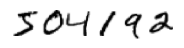
\includegraphics[scale=0.7]{img/mnist_example.png}
			\caption{Beispiele aus dem Datensatz MNIST \cite{mnist_data}}
			\label{fig:mnist}
		\end{figure}

	\subsection{Klassifikationsprobleme}

		Die allgemeine Problemstellung die ein \textit{Neural Network} lösen kann ist die folgende:\\
		Gegeben sei eine Zielfunktion $f:\mathcal{H} \to \mathcal{G}$.\\
		Da diese Funktion aber nicht bekannt ist, soll sie möglichst gut approximiert werden. \\
		Hierzu muss aus einer Menge von Funktionen $f_p:\mathcal{H} \to \mathcal{G}$ mit $p \in \Theta$ aus dem Parameterraum, diejenige ausgewählt werden, die $f$ am besten approximiert.
		In der Praxis ist es nicht leicht zu sagen, was es bedeutet, dass $f_p$ eine gute Approximation für $f$ ist.
		Für unsere Anwendung sind vorrangig Klassifaktionsprobleme interessant, hier enthält $\mathcal{G}$ alle verschiedenen Klassen und ist meistens endlich.
		Um in diesem Fall die Güte quantifizieren zu können, und um verschiedene Funktionen $f_p$ vergleichen zu können, definieren wir die Genauigkeit auf den Testdaten,
		die aus dem Englischen \textit{classification accuracy} auch kurz als \textit{Accuracy} bezeichnet wird:

		\begin{defi}[Classification accuracy] ~\\
			Zu der zu approximierenden Funktion $f$ betrachten wir eine Menge von $m$ Testdaten \\
			$(t_i, f(t_i)) \in \mathcal{G} \times \mathcal{H}$ $i \in \{1, \cdots , m\}$ mit korrekt klassifizierten Punkten $t_i$. \\
			Die Accuracy $acc$ ist nun definiert als:
			$$ acc(f_p) = \frac{1}{m} \sum_{k=1}^m \delta_{f(t_i)f_p(t_i)} \text{ wobei } \delta_{ij} =
			\begin{cases}
				1 & i = j \\
				0 & \, \text{sonst}
			\end{cases}$$
			Die Accuracy gibt also an welcher Anteil der Testdaten korrekt klassifiziert wird.
		\end{defi}

		Um geeignete Parameter aus $\Theta$ zu finden, ohne das wir die Testdaten verwenden dürfen, gibt es einen Trainingsdatensatz mit $n$ Daten
		$(x_i, f(x_i)) \in \mathbf{G} \times \mathbf{H}$ $i \in \{1, \cdots , n\}$, die ebenfalls bereits richitg klassifiziert sind.
		Aktuelle Methoden des machinellen Lernens optimieren nun die \textit{Accuracy} auf den Trainingsdaten, was auch die \textit{Accuracy} auf den
		Testdaten verbessert. Letzteres gibt nach dem Training an, wie gut der Klassifizierer neuen Daten vorhersagen kann
		und dient als Vergleichsmetrik zwischen mehreren Klassifizierern.\\

		Wenn wir erneut das Klasifaktionsproblem MNIST betrachten ergiben sich insgesamt z.B: \\
		$\mathcal{H} = \mathbb{R}^{28 \times 28}$, $\mathcal{G} = \{0, \cdots, 9\}$ sowie $n = 60.000$ Trainingsdaten und $m = 10.000$ Testdaten.


	\subsection{Neuronale Netze}\label{nets}
		
		\subsubsection{Neuronen}

			Um verstehen zu können was \textit{neurale Netzte} (im Verlauf auch kürzer \textit{Netze} genannt) sind, schauen wir uns zuerst den Grundbaustein an, aus denen sie bestehen,
			die (\textit{künstlichen}) \textit{Neuronen}.
			Ein Neuron ist eine kleine Einheit die eine Menge Inputs $x_1, \cdots, x_n$ erhält und daraus einen Output $y$ berechnet.
			Graphisch lässt sich das folgendermaßen vorstellen:

			\begin{figure}[h]
				\centering
				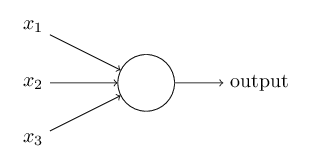
\includegraphics[scale=0.7]{img/neuron.png}
				\caption{Ein Neuron \cite{textbook}}
				\label{fig:neuron}
			\end{figure}

			\begin{defi}[Neuron] ~\\
				Mathematisch gesehen handelt es sich bei einem Neuron um eine Funktion\\
				$y = g(\mathbf{x}) = \sigma(\sum_{j=1}^n \omega_jx_j + b)$ wobei $\sigma$ die Aktivierungsfunktion des Neurons ist.
			\end{defi}

			$\omega_j$ und $b$ sind dabei die Gewichte und der Bias des Neurons, diese beiden beinflussen, was genau das Neuron berechnet und müssen trainiert werden.
			Sie sind also Teil des Parameterraums $\Theta$ eines neuronalen Netzes.
			Sobald sie einmal festgelegt wurden ändern Sie sich jedoch nicht mehr, sind also unabhängig von $\mathbf{x}$.
			Welches $\sigma$ gewählt wird beeinflusst, wie sich ein Netzt beim Training verhält und wird problemspezifisch angepasst.
			Es handelt sich um den ersten Hyperparameter, der beeinflusst wie die Funktion $f_p$ für ein festes $p \in \Theta$ aussieht. Dazu später mehr.
			In der Praxis werden zwei Aktivierungsfunktionen häufig verwendet, Die Sigmoid- und die ReLU-Aktivierungsfunktion:

			\begin{defi}
				Die Sigmoidfunktion ist definiert als
				$$sig(z) \coloneqq \frac{1}{1+e^{-z}}$$
			\end{defi}
			\begin{defi}
				Eine weitere Funktion ist die ReLU-Funktion:
				$$ReLU(z) = \max(0, z)$$
			\end{defi}

			Beide Funktionen haben Eigenschaften die sie zu guten Kandidaten für Aktivierungsfunktionen machen, da sie das schnelle und effektive Trainieren von neuronalen Netzten ermöglichen.

		\subsubsection{Fully Connected Layer}

			Ein neuronales Netzt besteht aus sogenannten \textit{Layern} von Neuronen. Das sind Schichten die viele Neuronen enthalten, die nicht untereinander, aber mit den
			Neuronen der benachbarten Schichten, bzw \textit{Layern} verbunden sind. \\
			Eine \textit{Layer} fasst also die einzelnen Funktionen der $m$ Neuronen $g_i$ zu einer großen Funktion $g$ zusammen.
			$g$ operiert auf einem Vektor $\mathbf{X}$, der als Komponenten alle Ouputs der vorherigen Layer enthält.
			Jedes $g_i$ enthält immernoch seine eigenen Parameter $\omega_1^i, \cdots, \omega_n^i$ und $b^i$.
			
			In normalen neuronalen Netzten gibt es nur sogenannte \textit{Fully Connected Layer} oder \textit{Dense Layer}, das sind \textit{Layer}, bei denen der Output jedes Neurons
			einer der Inputs jedes Neurons in der nächsten \textit{Layer} ist. Die beiden \textit{Layer} sind also vollständig miteinander verbunden.
			Eine \textit{Fully Connected Layer} mit $m$ Neuronen und Funktionen $g_1, \cdots, g_m$ hat also die oben angesprochene Funktion\\
			$$g(\mathbf{X}) = (g_1(\mathbf{X}), \cdots, g_m(\mathbf{X}))^T$$

			Der Input der ersten Layer von Neuronen ist $\mathbf{x} \in \mathcal{H}$. Die einzelnen Komponenten von $\mathbf{x}$ bilden ebenfalls eine \textit{Layer},
			die sogeannte \textit{Input Layer}. Die letze \textit{Layer} aus Neuronen heißt auch \textit{Output Layer}, da ihr Output die Komponenten von $f_p(\mathbf{x}) \in \mathcal{G}$ darstellt.
			Jede anderen \textit{Layer} von Neuronen heißt \textit{hidden (versteckte) Layer}. Schon mit nur einer \textit{hidden Layer} kann man jede stetige Funktion
			z.b. bzgl. $\norm{\cdot}_{sup}$ mit steigender Anzahl an Neuronen beliebig gut approximieren.
			Dieses \textit{Universalitätstheorem} erklärt, warum sich neuronale Netze in so unterschiedlichen Problemen anwenden lassen.

			Im Fall unseres MNIST Datensatzes wäre z.B. ein einfaches Netzwerk mit einer \textit{hidden Layer} denkbar:

			\begin{figure}[h]
				\centering
				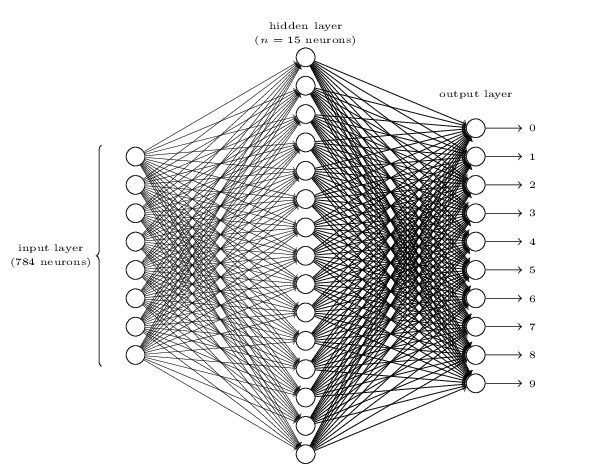
\includegraphics[scale=0.7]{img/mnist_net.png}
				\caption{Teilausschnitt aus einem neuronalen Netz \cite{textbook}}
				\label{fig:layer}
			\end{figure}
			
		\subsubsection{Convolutional Layer}

			Da sich das Hauptaugenmerk unseres Algorithmus auf Klasifaktionsproblemen in der Bilderkennung liegt, betrachten wir zudem die dort üblichen \textit{Convolutional Neural Networks}.
			Dises erweitern die Idee der neuronale Netze um eine weitere Art zwei \textit{Layer} zu verbinden - die Faltung, im Englischen \textit{Convolution}.
			Anders als bei den vollständig verbunden \textit{Layern} werden nur die räumlich lokalen Nachbarn zusammengefasst. Das heißt, der Output eines Neurons ist nicht für jedes Neuron der nächsten
			\textit{Layer} ein Input, sondern nur für manche (räumlich nahe). Außerdem hat nicht jedes Neuron seine eigenen Gewichte $\omega_j$ sondern es gibt einen Faltungskern (\textit{Kernel}),
			der bestimmt, wie die einzelnen Inputs gewichtet werden.
			Wir betrachten nur die zweidimensionale Faltung, dafür müssen die einzelnen \textit{Layer} nicht eindimensional wie in \ref{fig:layer}
			sondern zweidimensional angeordnet werden. \\
			Sei $\mathbf{X} \in \R^{m \times n}$ der Input der \textit{Layer}. Im Gegensatz zu einer \textit{Fully Connected Layer} wo\\
			$$g(\mathbf{X})_{ij} = g_{ij}(\mathbf{X}) = \sigma(\sum_{k_1=1}^m \sum_{k_2=1}^n \omega_{k_1k_2}^{ij}\mathbf{X}_{k_1k_2} + b^{ij})$$
			gelten würde, gibt es nun einen Faltungskern $K \in \R^{\hat{m} \times \hat{n}}$ und es gilt
			$$g(\mathbf{X})_{ij} = g_{ij}(\mathbf{X}) = \sigma(\sum_{k_1=1}^{\hat{m}} \sum_{k_2=1}^{\hat{n}} K_{k_1k_2}^{ij} \mathbf{X}_{i + k_1 - 1, j + k_2 - 1})$$
			Oft wird zudem $\sigma(z) \coloneqq z$ gewählt, bzw. kein $\sigma$ verwendet.
			Intuitiv lässt sich die Faltung so interpretieren, dass der Faltungskern über den Input läuft und an jeder Stelle einen Output generiert. Dieser Vorgang ist hier noch einmal dargestellt:

			\begin{figure}[h]
				\centering
				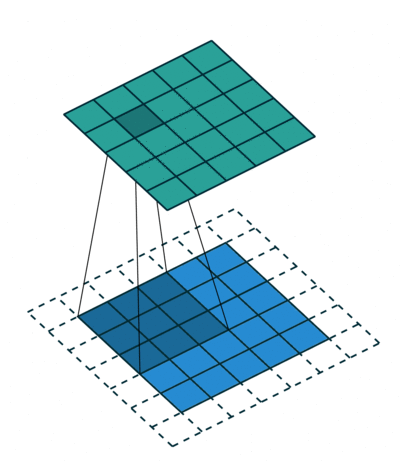
\includegraphics[scale=0.7]{img/convolution.png}
				\caption{grapische Darstellung einer Faltung mit Faltungskern $K \in \R^{3 \times 3}$ \cite{convo}}
				\label{fig:convo}
			\end{figure}

			Es fällt zudem auf, dass die Größe von $g(\mathbf{X})$ nun nicht mehr beliebig gewählt werden kann, wie bei der \textit{Fully Connected Layer}, stattdessen ist die Größe durch die Faltung
			eindeutig bestimmt. Es gilt $g(\mathbf{X}) \in \R^{m' \times n'}$ mit $m' = m - \hat{m} + 1$ und $n' = n - \hat{n} + 1$.

			Die Gewichte $K$ des Faltungskerns werden trainiert und sind Teil des Parameterraums $\Theta$ während $\hat{m}$ und $\hat{n}$ Hyperparameter sind.
			Zudem gibt es noch weitere Hyperparameter wie \textit{stride} oder \textit{padding}. Für mehr Informationen siehe \cite{convo}.

		\subsubsection{Pooling Layer}
			In \textit{Convolutional Neural Networks} gibt es noch eine dritte Art zwei \textit{Layer} zu verbinden, die \textit{Pooling Layer}.
			Sie ähnelt der \textit{Convolutional Layer}, statt mit einem Faltungskern werden räumlich nahen Inputs mit einer anderen
			einfachen Funktion verknüpft:
			\begin{align*}
				g&(\mathbf{X})_{ij} = g_{ij}(\mathbf{X}) \\
				= p&ool(\mathbf{X}_{i, j}, \cdots, \mathbf{X}_{i, j + \hat{n} - 1}, \mathbf{X}_{i + 1, j}, \cdots, \mathbf{X}_{i + 1, j + \hat{n} - 1},
				   \cdots, \mathbf{X}_{i + \hat{m} - 1, j}, \cdots, \mathbf{X}_{i + \hat{m} - 1, j + \hat{n} - 1})
			\end{align*}
			Dies ist meistens das Maximum oder der Durschnitt. Man spricht von \textit{Maximum Pooling Layer} oder \textit{Average Pooling Layer}.

	\subsection{Parameter und Training}\label{train}
		Wir haben nun gesehen, das neuronale Netze eine Funktion $f_p$ darstellen, die von Gewichten und Bias, also den Parametern $p \in \Theta$ abhängt.
		Diese Parameter sind die trainierbaren Parameter des neuronalen Netzes und unterscheiden sich so von den nicht trainierbaren Hyperparametern.
		Das Ziel besteht nun $p$ möglichst gut bezüglich der Trainingsgenauigkeit (\textit{Accuracy}) zu wählen. Das geschieht mit iterativen Lernverfahren, die ausgehend von initialen Anfangsparametern 
		immer bessere $p$ erzeugen. Diesen iterative Vorgang nennt man "trainieren". \\
		Dazu werden oft auf dem Gradientenabstieg (\textit{Gradiant Descent}) basierende Methdoden verwendet, die eine Kostenfunktion über $p$ minimieren,
		die angibt wie gut $f_p$ die Trainingsdaten vorhersagen kann. Für das Lernen bieten aktuelle Bibliotheken bereits vorgefertigte Optimierer, wie z.B.
		in \textit{PyTorch} den \textit{Stochastic gradiant descent} (\textit{SGD}) oder den Optimizier \textit{ADAM}. \\
		Alle Optimierer müssen mit verschiedenen Hyperparametern wie einer \textit{learning rate} eingestellt werden, die beispielsweise angibt wie schnell/fein sich $p$ verbessert. \\
		Ohne zu viel auf diese Hyperparameter eingehen zu wollen ist klar, dass die Auswahl dieser Hyperparameter ein gewisses Verständnis des Optimierers voraussetzt und einen
		großen Einfluss auf die Trainingsgeschwindigkeit und Güte des Ergebnisses hat. \\

		Zusätzlich gibt es noch weitere nicht trainierbare Hyperparameter, darunter unter anderem die Anzahl und Art von \textit{Layern} und welche \textit{Layer} untereinander verbunden sind.
		Man spricht hier oft von der Topologie des Netzes. Des weiteren gibt es noch die Hyperparameter der einzelnen Layern wie
		die Anzahl der Neuronen (bei einer \textit{Fully Connected Layer}) oder die Größe des Faltungskerns (bei einer \textit{Convolutional Layer}). \\
		All diese Hyperparameter des Netzes ändern $\Theta$ und wie $f_p$ für ein festes $p \in \Theta$ aussieht.
	
	\subsection{Hyperparametersuche}
		Insgesamt gibt es also jede Menge Hyperparameter, die gewählt werden müssen und ein Vielzahl von möglichen Topologien. Ohne gründliches Wissen über neuronale Netze
		ist es für den Einsteiger sehr schwer geignete Hyperparamter zu finden. Erfahrungen aus der Praxis zeigen, in welchen Situation welche Werte sinnvoll sind.
		Mit genügend Erfahrung kann man strukturiert verschiedene Hyperparameter austesten. Diese durch Erfahrung gewonnen Erkenntnisse und weitere Ratschläge finden sind zum Beispiel in dem Paper
		"Practical Recommendations for Gradient-Based Training of Deep Architectures" von Yoshua Bengio \cite{parameters}.\\

		Einem Anwender, der sich mit neuronale Netzen nicht gut auskennt, sollte es aber im besten Fall erspart werden, sich so tief in die Materie einlesen zu müssen.
		Obwohl moderne Bibliotheken wie \textit{PyTorch} mit bereits implementierten Methoden und Klassem viele lästige und komplizierte Aufgaben bereits abnehmen,
		und so auch Nicht-Experten das Experimentieren mit neuronalen Netzen ermöglicht wird, wäre es wünschenswert auch die Wahl der Hyperparameter zu automatisieren.\\

		Das Ziel ist es, dass der Anwender nur deklarativ die Trainings- und Testdaten angibt und ein Algorithmus automatisch das passende Netz auswählt und
		es trainiert, so dass mit genügend Rechenzeit auch ohne Expertise ein gutes Resultat ensteht.
		Auch wenn man schon alles über neuronale Netze weiß ist dies trotzdem erstrebenswert, da so mehr Zeit für wichtigere Aufgaben bleibt,
		während die immer besser werdenden Computer die Rechenarbeit übernehmen. \\
		Diesen Algorithmus zu entwickeln war meine Aufgabe im Fachpraktikum und das Resultat ist der Algorithmus \textit{convNEAT}.

	\subsection{bisherige Ansätze}\label{ansatz}

		Aufgrund der Bedeutendheit der Hyperparametersuche ist es nicht verwunderlich, dass schon viele Anstrengungen in diese Richtung unternommen werden.
		Wir betrachten nun ein paar klassische Ansätze der Hyperparametersuche, wie sie auch in \cite{parameters} beschrieben werden.
		Allen Ansätzen ist es gleich, das viele Netze nacheinander trainiert werden müssen. Danach wählt man das beste aus allen betrachtenden Netzen.

		\subsubsection{Grid Search}\label{grid}

			Für jeden Parameter der gewählt werden soll kan man ein Intervall angeben, in dem nach dem optimalen Wert des Parameter gesucht werden soll.
			So kann man den Suchraum definieren, in dem man nach den besten Hyperparametern suchen möchte.
			
			Die Idee des \textit{Grid Search} ist es nun für jedes dieser Werteintervalle ein Liste diskreter Werte auszuwählen.
			Für jede Kombination aus möglichen Werten, lässt man nun einmal das entstehende Netz trainieren, bis schlussendlich die besten Hyperparameter gefunden wurden.

			Durch geschicktes Design kann \textit{Grid Search} noch verbessert werden, z.B. indem man bei der Auswahl der Werte aus dem Werteintervall
			Wissen einfließen lässt, wie z.B. dass sich die \textit{learning rate} des Optimizers für ähnliche Größenordnungen auch ähnlich verhält und 
			man deshalb besser logarithmisch linear Werte auswählt also z.B. [0.1, 0.01, 0.001, 0.0001].
			Auch kompliziertere Erweiterungen wie geschatelte Suchen mit immer höherer Auflösung oder portionsweise
			nur ein paar Hyperparameter auf einmal zu testen und dafür mehrere Tests durchzuführen, kann die Güte und Geschwindigkeit des Verfahrens verbessern.
			Für weitere Details siehe \cite{parameters}.

			Trotzdem bleibt \textit{Grid Search} sehr rechenaufwändig, da die Anzahl an Tests exponentiell in der Anzahl der Hyperparameter ist.


		\subsubsection{Random Search}

			Im Gegensatz zur \textit{Grid Search}, die systematisch den Suchraum absucht kann durch die zufällige Wahl von Hyperparametern erstaunlicherweise
			viel schneller und soagar bessere Ergebnisse erzielt werden. \cite{randomsearch}
			Für jeden Parameter wird eine Verteilung angeben, meistens eine Gleichverteilung über das logaritmische Werteintervall (siehe \ref{grid})
			oder eine multinomiale Verteilung bei diskreten Hyperparametern.

		\subsection{NEAT}

			Einen ganz anderen Ansatz verfolgen sogenannte genetische Algorithmen. Sie basieren auf den drei genetischen Operatoren \textit{Mutation}, \textit{Selektion} und \textit{Crossover}.
			Ähnlich zur Evolution in der Natur wird eine Population verwaltet. Die einzelnen Individuen können mutieren, durch evolutionären Druck aussortiert werden und aus zwei
			Individuen können Nachkommen generiert werden, die Teile der Gene der Eltern besitzen.
			
			Für die Hyperparameterwahl ist besonders das Paper "Evolving Neural Networks through Augmenting Topologies" \cite{neat} aus dem Jahr 2002 hervorzuheben, das den Grundstein für alle vergleichbaren Methoden gelegt hat.
			Die Idee ist simpel. Um eine bestmögliche Netztopologie zu finden, kann man mit einem möglichst kleinen, einfachem Netz anfangen und durch Mutation und Crossover
			neue immer größere Netze erzeugen, die immer besser werden. Sobald die enstehenden Netze nicht mehr besser werden kann man aufhören.

			Ein Nachteil an NEAT ist jedoch, dass der Algortihmus in einer Zeit entwickelt wurde, als die Computer noch nicht so viele Möglichkeiten hatten wie heutzutage
			und außerdem zeitdem viele Fortschritte im Bereich des machinellen Lernens gemacht wurden, die bei \textit{NEAT} nicht berücksichtigt werden konnten.
			In \textit{NEAT} werden einzelne Verbindungen und Neuronen erzeugt und mutiert. \textit{NEAT} ist nicht darauf ausgelegt moderne Netze
			mit mehreren Tausend Neuronen zu erzeugen, sondern nur höchstens ein paar Hundert. Das ist für aktuelle Zwecke nicht mehr ausreichend.
			Außerdem sieht \textit{NEAT} vor, dass auch die Parameter in $\Theta$ durch Evolution trainiert werden. Hierfür stehen
			mittlerweile viel bessere und performantere Methoden wie \textit{SGD} oder \textit{ADAM} zur Verfügung. \ref{train}

	\clearpage

	\section{convNEAT}

		\textit{NEAT} liefert die Grundidee für den entwickelten Algorithmus. \\
		Wir übertragen das Konzept in die Moderne, in dem wir nicht mit einzelnen Neuron arbeiten,
		sondern als Grundeinheit ganze \textit{Layer} von Neuronen betrachten und auf und zwischen diesen Mutationsperationen definieren. \\
		Das Training auf den Trainingsdaten überlassen wir einem moderneren Optimierer wie in \ref{train}.
		Zusätzlich betrachten wir nicht nur neurale Netze sondern auch \textit{Convolutional Neural Networks} die unserem Algorithmus den Namen \textit{convNEAT}
		verleihen. So können wir besonders Klasifaktionsprobleme in der Bildverarbeitung wie den MNIST Datensatz \ref{mnist} besser lösen. \\

		Es gibt bereits ähnliche Versuche die Ideen von \textit{NEAT} auf \textit{Convolutional Neural Networks} zu übertragen, wie etwa
		\textit{EXACT} von T. Desell \cite{exact} oder \textit{EvoCNN} von Y. Sun et al \cite{convoneat}.
		Beide Ansätze haben Nachteile gegenüber \textit{convNEAT}, zeigen aber, dass ein genetischer Ansatz durchaus zielführend sein kann. \\
		Sie verwenden keine Kapselung der Netze in Species wie bei \textit{NEAT} und erlauben beide nur begrenzte \textit{Convolutional Neural Networks}.
		ConvNEAT bietet eine größere Flexibilität und mehr Möglichkeiten für beliebige \textit{feedforward Convolutional Neural Networks}
		auch mit \textit{Pooling Layern}, sowie leichte Erweiterbarkeit und Anpassbarkeit. Durch modernes \textit{Clustering} können
		bessere Ergebnisse erzielt werden und durch die Evolution von allen Hyperparametern inklusive den Hyperparametern des Optimierers
		werden dem Anwender alle schwierigen Entscheidungen abgenommen.\\

		Die Grundidee von \textit{convNEAT} ist im folgenden kurz als Pseudocode dargestellt.

		\begin{algorithm}
			\caption{\textit{convNEAT}}\label{pseudo}
			\begin{algorithmic}
				\State \textit{population} $\gets$ Initialisiere die Startpopulation mit einfachen Netzen
				\While{durschnittliche Accuracy verbessert sich}
					\State Trainiere alle Netze aus \textit{population} und bestimme ihre Accuracy
					\State \textit{parents} $\gets$ Selektiere Paare von Netzen aus \textit{population}
					\State \textit{population} $\gets$ Generiere mit \textit{Crossover} neue Netze aus allen Paaren in \textit{parents}
					\State Mutiere alle Netze aus \textit{population}
				\EndWhile
			\end{algorithmic}
		\end{algorithm}
		
		Bevor wir auf weitere Details von \textit{convNEAT} eingehen, werden wir zuerst ein grundlegendes Probleme ansprechen.

		\subsection{Representation}

			Da wir mit einem evolutionären Algorithmus arbeiten, müssen wir eine geieignete genetische Representation finden.
			Diese Kodierung des Netzes als \textit{Genom}, bestehend aus mehreren Genen, bestimmt wie das Netz aussieht, und muss deshalb alle Hyperparameter enthält die uns interessieren.
			Neben der Anzahl und der Größe der \textit{Layer}, so wie deren Hyperparameter, gehören aber auch alle anderen Hyperparameter, z.B. 
			die des Optimieres dazu.

			Die Representation bestimmt schlussendlich welche Netze gebildet werden können, also auch den Suchraum in dem gesucht werden muss.
			Dieser Suchraum kann dank des evolutionären Ansatzes viel größer sein als bei einer \textit{Grid Search} oder \textit{Random Search} \ref{ansatz}.
			\textit{EvoCNN} verwendet z.B. eine Liste von \textit{Layern} variabler Länge um Netze darzustellen.
			Der Suchraum ist beschränkt auf diejenigen \textit{Convolutional Neural Networks}, die erst eine Reihe \textit{Convolutional Layer}
			und danach eine Reihe von \textit{Fully Connected Layer} aufweisen. 

			\textit{convNEAT} schränkt den Suchraum nicht so weit ein, sondern lässt alle möglichen \textit{feedforward Convolutional Neural Networks} zu.
			Gerade für schwierige Probleme und Netzen mit vielen \textit{Layern} reichen einfache Netze wie in \textit{EvoCNN} nicht aus \cite{deep}.

			convNEAT verwendet eine Kodierung, die an die Kodierung in \textit{NEAT} angelehnt ist.
			\textit{NEAT} kodiert neuronale Netze als Graph, wobei die Neuronen die Knoten und die Verbindungen mit Gewichten die Kanten sind.
			Natürlich muss dieser Ansatz angepasst werden, trotzdem kann man sich jedes \textit{Convolutional Neural Net},
			also auch jedes gewöhnliche neuronale Netz als einen Graphen vorstellen: \\
			Die Knoten sind die einzelnen \textit{Layer} und die Verbindungen zwischen den einzelnen \textit{Layern} werden über die Kanten beschreiben.
			Wie wir bereits in \ref{nets} gesehen haben hängt letzteres davon ab, um was es sich bei der hinteren \textit{Layer} handelt.
			Diese Information, ob \textit{Fully Connected Layer}, \textit{Convolutional Layer} oder \textit{Pooling Layer}, ist zusammen mit allen
			zugehörigen Hyperparametern in den Kanten gespeichert.

			Wie bereits erwähnt ist die Anzahl der Neuronen in den Knoten nicht immer frei wählbar, sondern nur falls es sich bei der eingehenden Kante
			um eine \textit{Fully Connected Layer} handelt. Aus diesem Grund wird die Größe nicht in den Knoten kodiert.
			Stattdessen wird die Größe des Inputs durch das Netz propagiert und in jeder Kante bearbeitet. Für \textit{Fully Connected Layer} wird gespeichert
			wie groß die Änderung der Größe ist, also zum Beispiel, dass die nächste \textit{Layer} 20 mehr Neuronen enthält als ihr Vorgänger.
			Es können auch inaktive Kantengene in Genom gespeichert werden, die einfach ignoriert werden.

			Wenn wir beliebige gerichtete Graphen zulassen stoßen wir auf zwei Probleme:
			Es kann zu Kreisen kommen, so dass das Durchpropagieren des Inputs nicht mehr funktioniert. \\
			Diesem Problem können wir entgegenwirken, in dem wir beim Hinzufügen einer Kante darauf achten, dass keine Kreise enstehen. \\
			Außerdem ist es möglich, dass ein Knoten zwei eingehende Kanten besitzt, die verbunden werden müssen.
			In diesem Fall müssen durch Hochskalierung, Runterskalierung, einer Mischung aus beiden oder durch das Hinzufügen von Nullen die 
			Ouputs auf die selbe Größe gebracht und konkatiniert werden. Wie genau das passiert ist ein weiterer Hyperparameter der im Knoten kodiert wird.

			Für maximale Flexibilität besonders auf die Anwendung der Bildanalyse bezogen, sind alle \textit{Layer} im späteren Netz, dreidimensional.
			Neben Höhe und Breite gibt es noch verschiedende Channels, in denen z.B. im Input Gelb-, Rot- und Blauanteile kodiert werden könnten.
			Bei MNIST bleibt der Input dann z.B. $\mathbf{X} \in \mathbb{R}^{1 \times 28 \times 28}$.
			Das sorgt dafür, dass im Verleich zu z.B. \textit{EXACT} viel weniger Knoten gebraucht werden, weil viel mehr Faltungen kompakt
			representiert werden können. \\
			Neben der Topologie wird auch noch kodiert welcher Optimierer gerade mit welchen Hyperparametern verwendet wird.

			\begin{figure}[h]
				\centering
				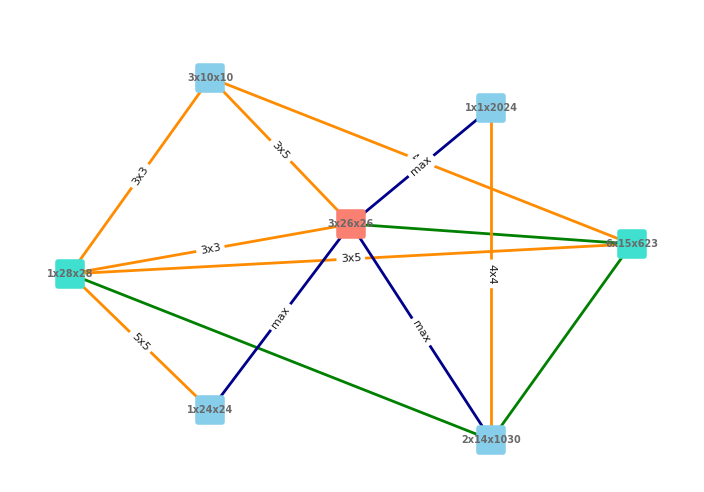
\includegraphics[scale=0.7]{img/net2.png}
				\caption{Ein Beispiel für ein komplexeres Netz das kodiert werden kann. Die Farben der Kanten geben ihren Typ an, z.B. steht orange für eine \textit{Convolution Layer}}.
			\end{figure}

		\subsection{Mutation}

			Die Möglichkeit Genome zu mutieren bildet die Basis jedes genetischen Algorithmuses, so können neue Netze erzeugt werden, die den
			bisherigen Netzen ähneln. Unvorteilhafte Mutationen können in der \textit{Selektion} aussortiert werden, gute Mutationen bleiben erhalten.
			Welche Mutationen enstehen ist zufällig, manche haben jedoch höhere Wahrscheinlichkeit als andere.
			Die Wahrscheinlichkeiten wurden durch viele Testläufe so angepasst, dass Sie sinnvoll sind.
			Diese Hyper-Hyperparameter von \textit{convNEAT} müssen nur einmal eingestellt werden und sind problemunabhängig.
			Trotzdem wäre es denkbar auch eine adaptive Veränderung der Wahrscheinlichkeiten einzubauen, um diejenigen Mutationen häufiger auftretten zu lassen,
			die häufiger zu guten Netzen führen.

			\textit{convNEAT} bietet folgende Mutationen:

			\begin{enumerate}
				\item [] \textbf{Aktivieren und Deaktivieren von Genen} \\
					Es besteht die Möglichkeit Gene zu deaktivieren und wieder zu reaktivieren. Deaktivierte Gene spielen keine Rolle mehr für das entstehende Netz.
					Deaktivierte Gene können auch durch den \textit{Crossover} \ref{cross} entstehen. Beim Deaktivieren muss sichergestellt sein, dass
					es noch einen Pfad vom Input zum Output gibt.

				\item [] \textbf{Kante aufteilen} \\
					Es besteht die Möglichkeit eine bestehende Kante aufzuteilen. Dabei entsteht ein neuer Knoten zwischen zwei existierenden Knoten.
					Die ursprüngliche Verbindungskante wird deaktiviert und zwei neue Kanten eingefügt. Die erste ist eine Kopie der alten Kante.
					Die zweite neue Kante ist eines zufälligen Typs. Manche Kanten sind hier wahrscheinlicher, z.B. ist hinter einer
					\textit{Convolutional Layer} eine neue \textit{Pooling Layer} am wahrscheinlichsten.

				\item [] \textbf{Kante einfügen} \\
					Zwischen zwei Knoten kann eine Kante eingefügt werden. Wie beim Aufteilen einer Kante ist die Art der Kante zufällig.
					Damit keine Kreise entstehen können, wird für jeden Knoten seine Tiefe im Netz gespeichert.
					Eine neue Kante zeigt dann immer auf die tiefere Kante, beliebige Pfade durchlaufen immer Knoten in echt absteigender Tiefe,
					Kreise sind unmöglich.

				\item [] \textbf{Optimierer} \\
					Welcher Optimierer verwendet wird und alle seine Hyperparameter können ebenfalls mutiert werden.
					Dies kann unter anderem die \textit{learning rate} oder der \textit{weight decay} sein.

				\item [] \textbf{Kante mutieren} \\
					Alle Kantentypen können ihre Hyperparameter mutieren, jede Mutation hat seine typspezifische Wahrscheinlichkeit.
					Unter anderem sind folgende Mutationen möglich:
					\begin{enumerate}
						\item [] \textbf{Fully Connected Layer} \\
							Die Aktivierungsfunktion und die Größenänderung können mutieren.
						\item [] \textbf{Convolutional Layer doer Pooling Layer} \\
							Die Weite, Höhe und Tiefe des Kernels sowie weitere Parameter wie unter anderem \textit{padding} oder \textit{stride} können mutieren.
					\end{enumerate}
			\end{enumerate}

		\subsection{Selektion}\label{select}
			
			Wichtig für jeden genetischen Algorithmus ist der Operator der \textit{Selektion}. Die besten Netze werden beibehalten und die schlechtesten,
			z.B. diejenigen die durch eine unvorteilhafte Mutation entstanden sind, sollten nicht weiter überleben.
			Ein gutes Maß für die Güte eines Netzes ist die \textit{Accuracy} auf den Testdaten. Da beim öfteren Vergleich der \textit{Accuracy} auf den Testdaten,
			aber die Gefahr des \textit{Overfittings} besteht, also die Chance, dass das Netz das Rauschen der Testdaten lernt und auf neuen Daten keine guten Vorhersagen macht,
			wird ein Teil der Trainingsdaten nicht zum Trainieren verwendet sondern als Validierungsdaten zurückgehalten.
			Bei der Selektion kann dann die \textit{Accuracy} auf den Validierungsdaten bestimmt und verglichen werden.
			Die Testdaten werden nur ganz am Ende verwendet um die Güte des finalen Ergebnisses aus \textit{convNEAT} zu überprüfen.\\

			Damit Netze die schon länger trainiert haben keinen Vorteil gegenüber frisch mutierten Netzen haben gibt es für jede trainierte Epoche eine Strafe.
			Die Strafe ist linear im logarithmischen Klassifikationsfehler.

			\begin{defi}[Log classification error] ~ \\
				Der logarithmische Klassifikationsfehler eines Netzes mit Accuracy $a$ ist definiert als \\
				$$ logerr(a) = \log_{10}(1 - a)$$
			\end{defi}
		
			Für ein Genome mit Accuracy $a$ und $n$ trainierten Epochen kann man einen modifizierten score berechnen mittels\\
			$$score(a, p) =  1 - 10^{logerr(a) + n * decay}$$
			Denn so gilt:
			$$ logerr(score(a, p)) = logerr(a) + n * decay$$

			Basierend auf diesem angepasstem \textit{score} können jetzt Paare aus Genomen gebildet werden die im nächsten Schritt, dem \textit{Crossover} kombiniert werden können.
			Es ist auch möglich, dass ein Paar aus zweimal dem gleichen Genom besteht. Dann wird der \textit{Crossover} übersprungen und es kommt nur zur \textit{Muatation} des Genoms.
			Es gibt viele Möglichkeiten diese Selektion durchzuführen. In \textit{convNEAT} sind mehrere Methoden implemtiert. \\
			Von einfachen Methoden, wie die simple Auswahl aller besten Genome \textit{(cutoff)}, oder der zufälligen Wahl, bei der jedes Genom eine Wahrscheinlichkeit
			proportional zu seinem \textit{score} hat \textit{(fps)}, bis hin zu komplizierteren Methoden wie der \textit{Tournament selection (ts)} bei der zufällig eine
			Gruppe von $k$ Genomen ausgewählt wird, von denen das Beste ausgewählt wird, oder der \textit{stochastic universal sampling (sus)} \cite{sus}.

			Welche Methode die beste ist, muss mit vielen Testläufen auf verschiedenen Problemen ausgetestet werden, da meine Rechenzeit aber limitiert war, konnte
			ich nur einige wenige Tests auf dem MNIST Datensatz durchführen. Hier schien es, als ob \textit{stochastic universal sampling}
			eine stabile und effektive Methode der Selektion ist.

			Wichtig ist das die Selektion auch ein paar schlechtere Netze überleben lässt. Denn vielleicht sind manche Netze nicht lange genug trainiert worden
			und zeigen ihr volles Potenzial nach etwas mehr Zeit. \textit{stochastic universal sampling} besitzt diese Eigenschaft.

			Um eine Intuition für die verschiedenen Selektionsfunktion zu bekommen sind in \ref{tab:select} die durschnittliche Auswahlwahrscheinlichkeit
			einiger Verfahren für ein Beispielpopulation $x_i$, $i \in \{1, \cdots, 15\}$ mit $score(x_i) = i^2$ angegeben.
			Man kann gut sehen, wie \textit{stochastic universal sampling} bessere Werte bevorzugt, aber auch schlechtere Werte noch berücksichtigt.

			\begin{table}[h]
				\centering
				\begin{tabular}{llllllllllllllll}
					\toprule
					& $x_1$ & $x_2$ & $x_3$ & $x_4$ & $x_5$ & $x_6$ & $x_7$ & $x_8$ & $x_9$ & $x_{10}$ & $x_{11}$ & $x_{12}$ & $x_{13}$ & $x_{14}$ & $x_{15}$ \\
					\midrule
					\textit{cutoff} & 0 & 0 & 0 & 0 & 0 & 0 & 0 & 0 & 0 & 17 & 17 & 17 & 17 & 17 & 17 \\
					\textit{fps} & 0 & 0 & 1 & 1 & 2 & 3 & 4 & 5 & 7 & 8 & 10 & 12 & 13 & 15 & 17 \\
					\textit{ts} & 0 & 0 & 0 & 1 & 2 & 4 & 5 & 7 & 8 & 10 & 11 & 12 & 13 & 13 & 13 \\
					\textit{sus} & 0 & 0 & 1 & 1 & 2 & 3 & 4 & 5 & 6 & 8 & 10 & 12 & 13 & 16 & 18 \\
					\bottomrule
				\end{tabular}
				\caption{Einige Selektionsfunktionen zu $score(x_i) = i^2$ , alle Werte in $\%$}
				\label{tab:select}
			\end{table}
				
		
		\subsection{Crossover} \label{cross}

			Eine weitere Operation in genetischen Algorithmen ist der \textit{Crossover}. Er erzeugt aus zwei Genomen ein neues Genom.
			Dieses neue Genome erhält kann Gene beider Eltern enthalten. \textit{convNEAT} verwendet, wie bei \textit{EXACT},
			die Parameter \textit{more fit parent crossover rate} und \textit{less fit parent crossover rate}.
			Diese beiden beschreiben wie viel Prozent des jeweiligen Genomes aktiviert bleiben soll.
			Gene (hier vor allem die Kanten), die beispielsweise nur im besseren Genom (mit höherem \textit{score} \ref{select}) vorkommen,
			werden mit Wahrscheinlichkeit gleich der \textit{more fit parent crossover rate} aktiviert übernommen.
			Alle anderen Gene werden deaktiviert insofern das möglich ist.

			Da die Eltern zwei beliebige Graphen sein können, ist es schwierig zu sagen, welche Gene gleich sind und wie die ungleichen Gene kombiniert werden sollen.
			Abhilfe schafft das Konzept der \textit{historical markers} aus \textit{NEAT}. Jedes Gen bekommt eine eindeutige Zahl, die \textit{innovation number} zugeordnet.
			Wenn durch Muatation neue Kanten oder Knoten entstehen, werden ihnen neue Zahlen zugeordnet.
			Möchte man zwei Genome vergleichen, kann man sich die \textit{Marker} anschauen und sieht sofort wie viele Genome gleich sind und wie
			unterschiedlich (im biologischen Sinne) die Genome sind.

			Ein simples Beispiel für einen Crossover findet sich in in \ref{fig:crossover}

			\begin{figure}[h]
				\centering
				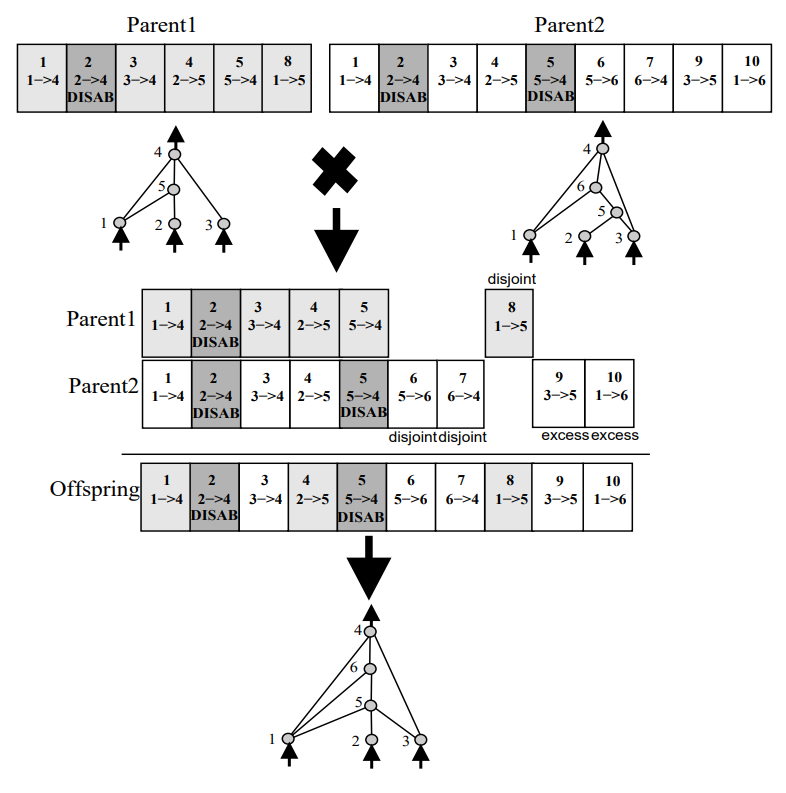
\includegraphics[scale=0.6]{img/crossover.png}
				\caption{Ein Beispiel für Crossover zweier Graphen aus \cite{neat}}
				\label{fig:crossover}
			\end{figure}

		\subsection{Clustering}

			Mit den obigen genetischen Operatoren ist bereits das Grundgerüst für \textit{convNEAT} entworfen.
			Theoretisch werden die Netze immer komplizierter und dadurch auch besser.
			In der Praxis tritt man jedoch auf ein Problem, das schon bei der Entwicklung von \textit{NEAT} bekannt war.
			Wird ein neues Netz generiert, z.B. durch \textit{Crossover} so kann es in der Praxis oft nicht lange überleben, es wird durch die Selektion
			schnell wieder aussortiert. Das neue Netz braucht nämlich einige Zeit um durch Training, oder weitere Mutationen langsam besser zu werden, bis es
			kompetetiv genug ist, um mit den aktuell besten Netzen verglichen werden zu können, die schon über viele Generationen optimiert wurden.

			Eine Lösung für das Problem ist wie \textit{EvoCNN} eine Selektion auszuwählen, die nur sehr geringen
			\textit{Selektionsdruck} ausübt, also auch schwache Netze oft überleben lässt. Da aber mit Senkung des \textit{Selektionsdruck}
			auch die Geschwindigkeit sinkt, mit der Fortschritte gemacht werden können, verwendet \textit{convNEAT} stattdessen das Konzept
			der \textit{Artentrenung} (im Englischen \textit{Speciation}), im weiteren auch mit \textit{Clustering} bezeichnet.

			Ähnliche Netze mit ähnlicher Topologie werden in einzelne \textit{Arten} (\textit{Cluster})zusammengefasst, so dass Netze im gleichen
			Cluster möglichst ähnlich und in verschiedenen Cluster möglichst verschieden sind.
			Die Selektion erfolgt jetzt nur innerhalb den einzelnen Clustern, so dass es dauerhaft Cluster von Netzen geben kann, die sich von dem besten Cluster unterscheiden.
			Während das beste Cluster weiter optimiert wird gibt \textit{convNEAT} auch anderen Ansätzen die Chance weiter erforscht und optimiert zu werden.

			Das Zusammenspiel der einzelnen Cluster untereinander muss genau geregelt sein. \textit{convNEAT} sorgt dafür, dass
			die besten Cluster größer werden können, um mehr Rechenzeit in die Optimierung der aktuell besten Lösung zu investieren, aber gleichzeitig andere
			Cluster nicht zu klein werden, auch wenn sie schlechter sind. Cluster die sich nicht weiter verbessern, weil die Netztopolgie einfach
			nicht passend für das Problem ist, werden nach einer gewissen Zeit gelöscht.

			Damit \textit{Clustering} funktionieren kann brauchen wir zwei Dinge: Eine Abstandsfunktion und einen Clusteralgorithmus.

			\subsubsection{Ähnlichkeit}

				Das Konzept von \textit{"ähnlichen"} Genomen muss nun mathematisch definiert werden.
				Für jede Art von Gen wird ein Ähnlichkeitsfunktion $sim(x, y) \in [0, 1]$ definiert, die angibt wie unterschiedlich
				die Hyperparameter sind. $sim(x,y) = 0$ bedeutet, dass die Ausprägungen $x$ und $y$ des Gens gleich sind. Je näher $sim(x,y)$ der $1$ ist, desto verschiedener sind die beiden Ausprägungen.

				\begin{defi} [Distanzmetrik]
					\textit{convNEAT} verwendet folgenden Abstand: \\
					$$dist = c_0*S + c_1*D + c_2*E + c_3*T + c_4*K + c_5*X$$
					wobei $S$ der Unterschied in den gemeinsamen Kanten ist, \\
					$D$ und $E$ zusammen die Anzahl der Gene die nur in einem der beiden Genome vorkommt, \\
					$T$ ist der Unterschied der verwendeten Optimierer, $K$ der Unterschied in den Knoten und $X$ der Unterschied in der Anzahl der trainierten Epochen.
				\end{defi}
				
				Diese Abstandsfunktion sorgt dafür, dass alle Unterschiede eine festlegbare Rolle spielen.
				Die Parameter $c$ wurden durch Testläufe optimiert. Am wichtigsten sind $S$, $D$ und $E$.

			\subsubsection{Clusteralgorithmus}
				
				Das Problem, eine Menge von $n$ Daten $\mathbf{X} \in \mathcal{A}^n$ in $k$ Cluster einzuteilen lässt sich als Optimierungsproblem darstellen. Zu minimieren ist der
				Abstand der Mitglieder der Clusters $S_i$ zum jeweiligen Clustermittelpunkt $\mu_i$:

				\begin{defi}
					$$J \coloneqq \sum _{i=1}^{k}\sum _{x_j \in S_i} dist(x_j, \mu_i)^2$$
				\end{defi}

				Für den Fall $\mathcal{A} = \mathbb{R}^m$ gibt es hervorragende Algorithmen wie \textit{k-Means} \cite{kmeans}, um das Optimierungsproblem
				approximativ sehr schnell zu lösen. \textit{k-Means} ist ein iteratives Verfahren, dass ausgehen von Start-Clustermittelpunkten $\mu_i^0$
				immer bessere $\mu_i$ findet, in dem es den Mittelpunkt der aktuellen zu Cluster $S_i$ gehörenden Datenpunkte zum neuen $\mu_i$ macht bis dieser Prozess konvergiert.

				Leider lässt sich \textit{k-Means} nicht auf unser Problem anweden, da der Suchraum kein Vektorraum mit einer Basis ist,
				der Begriff eines Mittelpunktes ist nicht defniert. Wir dürfen lediglich mit der Metrik $dist$ arbeiten.

				\textit{convNEAT} verwendet deshalb eine stark modifizierte Variante des \textit{k-Medoid} Algorithmuses.
				Im Gegensatz zum Mittelpunkt wählen wir den \textit{"Median"}, in unserem Fall das Genom im Cluster, dass den geringsten Abstand zu allen anderen
				Clustermitgliedern hat, also $$med(z) \coloneqq \sum _{x_j \in S_i} dist(x_j, z)$$ minimiert.

				\textit{k-Medoid} kann deshalb so umgebaut werden, dass es nur von $dist$ abhängt.
				Einige Dinge sind noch zu beachten, z.B. darf kein Cluster zu klein werden, da sonst keine sinnvolle Selektion stattfinden kann.
				Damit man messen kann wie sich die einzelnen Netze eines Clusters über die Zeit entwickeln muss zudem eine Art Konsistenz erhalten bleiben.
				Ist das Beste Cluster $S_k$ für ein festes $k$ dann sollte nach dem erneuten Clustern wieder viele Netze $x_j \in S_k$ im neuen Cluster $S'_k$ sein.
				Diese Konsistenz ist bei \textit{k-Medoid} nicht gegeben. Die Güte des Ergebnis im Bezug auf $J$ hängt stark von den Start-Clustermittelpunkten $\mu_i^0$
				ab. \textit{k-Medoid} wird deshalb üblicherweise mit verschiedenen kompliziert gewählten $\mu_i^0$ mehrmals ausgeführt.
				\textit{convNEAT} verzichtet auf eine komplizierte Initialiserung und verwendet stattdessen den Median der schon aus der letzten Generationen
				bekannten Cluster als Startwert. Die Einbüße in der Funktion $J$ können durch die enstehende Konsistenz gerechtfertigt werden.

				Der entwickelte \textit{consistent bounded k-Medoid} kann aber nur für festes $k$ eine Clusterung finden.
				Für \textit{convNEAT} ist es jedoch wichtig die Anzahl der Cluster varieren zu lassen, falls durch Mutation und Crossover viele
				neuartige Netze entstanden sind oder nach der Selektion zu wenige Netze eines Cluster übrig bleiben.

				\textit{convNEAT} ändert adaptiv die Anzahl der Cluster, falls dies nötig ist und achtet trotzdem darauf, dass die Konsistenz der Cluster erhalten bleibt.
				Ein Beispiel für die Ergebnisse des Clusterings finden sich in Abbildung \ref{fig:clust_ex} und \ref{fig:clust_d}.

				\begin{figure}[h]
					\centering
					\includegraphics[scale=0.58]{img/cluster_example.png}
					\caption{Die besten Netze aus zwei Clustern einer Population. Zu sehen ist ein Cluster mit simpleren Netzen mit einer
						\textit{Convolutional Layer} gefolgt von einer \textit{Fully Connected Layer} sowie Cluster mit komplexeren Netzen.}
					\label{fig:clust_ex}
				\end{figure}

				\begin{figure}[h]
					\centering
					\includegraphics[scale=0.6]{img/cluster.png}
					\caption{Die zu \ref{fig:clust_ex} gehörende Distanzmatrix $D$ mit $D_{ij} = dist(i, j)$.
						Blaue Farben zeigen eine hohe Ähnlichkeit an. Die rot umrandeten Teilmatrizen sind die clusterinternen Distanzen}
					\label{fig:clust_d}
				\end{figure}

		\subsection{Eliten und Training}
			
			Damit die Netze in der Population überhaupt gute Vorhersagen auf den Validierungsdaten machen können müssen sie auf den Trainingsdaten trainieren, dies geschieht in einer Trainingsphase.
			In dieser Phase kann jedes Netz eine feste Anzahl von Epochen auf den Daten trainieren. Die Laufzeit von \textit{convNEAT} ist auf diesen Schritt zurückzuführen, denn 
			wie bei der Arbeit mit neuronalen Netzen üblich, kann das Training sehr lange, manchmal Stunden oder Tage lang dauern.
			Wie schnell textit{convNEAT} zu einem Ergebnis kommt hängt also nur davon ab wie viele Epochen alle Netze gemeinsam trainiert werden.

			Netze die schnellen Fortschritt machen werden belohnt in dem Sie länger trainieren können. Dies sorgt dafür, dass insgesamt schnellerer Fortschritt gemacht wird.
			Besonders bei kompliziertern Problemen ist aber nicht klar, ob die festgelegte Anzahl an Epochen ausreicht um ein gutes Netz zu trainieren.
			Je nach Hyperparameterwahl dauert es eventuell viel länger. Die Netze hätten so überhaupt keine Zeit gut genug zu werden, um das Problem lösen zu können.

			Abhilfe schaffen die sogenannten \textit{Eliten}. Nach jeder Generation werden die besten Netze jedes Clusters automatisch in die nächsten Generation übernommen.
			Nur der verbleibende Platz in der Population wird durch den Crossover aufgefüllt.

			Das hat den Vorteil, dass die besten Netze die Möglichkeit haben über mehrere Generation so lange zu trainieren, wie sie brauchen um ihr Potenzial auszuschöpfen.
			Andererseits sorgt der angepasste score in \ref{select} dafür, dass Netze die schon länger trainiert haben, nicht bevorzugt werden und auch neue Netze noch die Chance haben
			sich zu etablieren. Zudem wird die Laufzeit gesenkt. Gute Netze die durch Training nich mehr zu verbessern sind, bleiben in der Population ohne jede Generation
			Trainingszeit zu verschwenden.
	
	\clearpage

	\section{Ergebnisse}\label{ergeb}
		
		Der entwickelte Algorithmus wurde in \textit{Python} implementiert und verwendet die Bibliothek \textit{PyTorch} um die Netze zu trainieren.
		Das entwickelte Modul lässt sich sehr einfach ausführen, der Einzige Input ist der Datensatz. 
		Alle Hyperparameter, wie die Anzahl der Genome in der Population kann eingestellt werden, aber auch die Standardwerte funktionieren bereits für die meisten Probleme.
		Zusätzlich zur detailierten Ausgabe im Terminal besitzt \textit{convNEAT} eine optionale graphische Oberfläche (siehe \ref{fig:gui}), die den aktuellen Trainingsfortschritt anzeigt und einen Überblick der Population gibt.
		Nach jeder Generation werden die besten Netze abgespeichert. Das Training kann dann unterbrochen und später fortgesetzt werden.
		Die Implementation kann online auf \href{https://github.com/Jukamala/convNEAT}{Github} abgerufen werden.
		Die Implementation bietet leichte Erweiterungsmöglichkeiten für andere \textit{Layer}-Typen, Optimierer oder \textit{score} Funktionen.

		Augrund der Tatsache, dass \textit{convNEAT} eine vergleichsweise lange Laufzeit besitzt und sehr viele Testläufe gemacht werden müssen um die Hyperparameter einzustellen, blieb nicht mehr genug Zeit
		\textit{convNEAT} auf verschiedenen Datensätzen zu testen und so die Vielseitigkeit von \textit{convNEAT} zu demonstrieren.
		Es wurden jeddoch einige Tests auf dem (leider etwas limitierten) MNIST Datensatz durchgeführt:

		\begin{figure}[h]
			\centering
			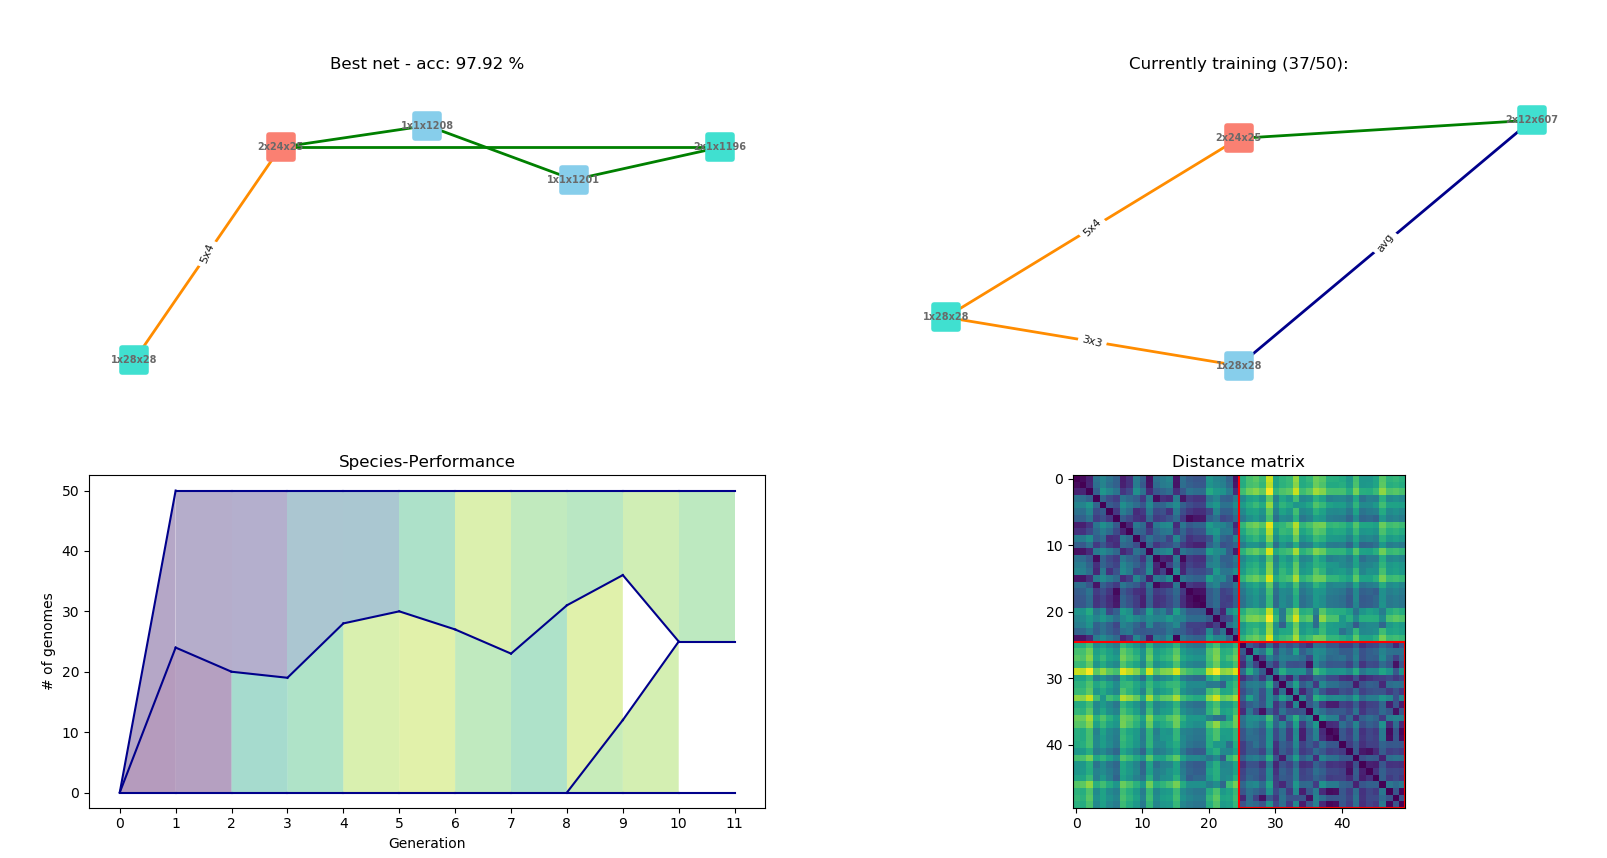
\includegraphics[scale=0.6]{img/dashboard.png}
			\caption{Die Öberfläche von \textit{convNEAT}. Neben dem besten und dem aktuell trainierten Netz findet
				sich hier eine Übersicht über die \textit{Performance} und die \textit{Clusterung}.
				Da MNIST keine sehr komplexer Datensatz ist, konnte auch eine einfache Topologie \textit{"gewinnen"}}
			\label{fig:gui}
		\end{figure}

		\clearpage

		\subsection{MNIST}
			
			Auf den Standardeinstellung erzeugt \textit{convNEAT} reltativ schnell Netze mit einer Accuracy von über $98 \%$ (je nach Seed sogar fast bis $99 \%$
			 und erfüllt damit die Ansprüche, die wir an den Algortihmus gestellt haben, automatisch ein passables Ergebnis zu erreichen.
			Die enstehenden Netze unterscheiden sich von Netzen die ein Mensch erstellen würde, sie sind viel organischer.
			In den Abbildungen \ref{fig:b1} und \ref{fig:b2} finden sich das besten Netz eines zufälligen Durchlaufs mit 15 Generation, so wie eine Übersicht über den Verlauf des Trainings.

			\begin{figure}[h]
				\centering
				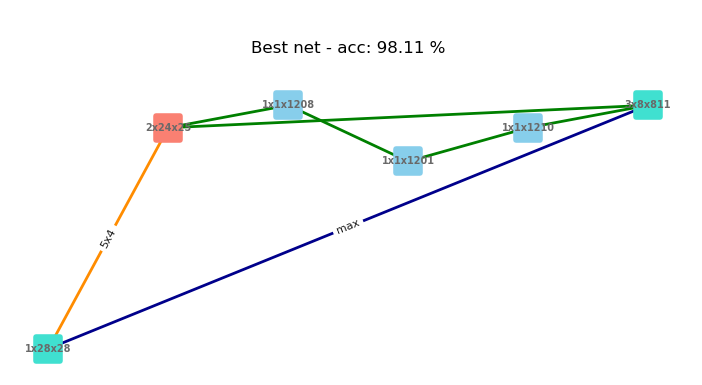
\includegraphics[scale=0.6]{img/bestnet.png}
				\caption{Das beste Netz mit einer \textit{Accuracy} von $98,11 \%$}
				\label{fig:b1}
			\end{figure}

			\begin{figure}[h]
				\centering
				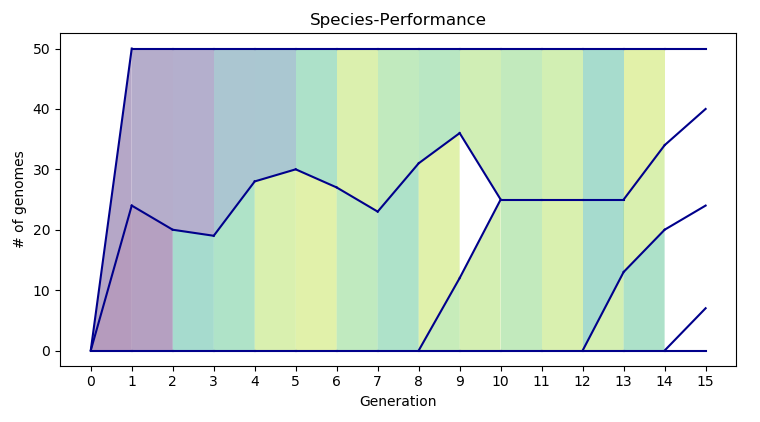
\includegraphics[scale=0.6]{img/verlauf.png}
				\caption{Eine grapische Darstellung des Verlaufes. Man erkennt die einzelnen Cluster mit apaptiv angepasster Größe. In der 10. Generation
						wird ein Cluster gelöscht, dass sich 3 Generationen lang nicht weiter verbessert hat.}
				\label{fig:b2}
			\end{figure}

			Wie in \ref{mnist} nachzulesen ist, ist MNSIT ein bereits \textit{"gelöstes"} Problem, bei dem schon Klassifizierer mit einer \textit{Accuracy} über $99.5\%$ existieren.
			Das letzte Prozent wird meist erst mit geieignetem Preprocessing der Daten erreicht.

			Vergleicht man die Resultate mit denen von \textit{EXACT}, so sieht man, dass die entstehenden Netze wie zu erwarten kompakter sind.
			\textit{EXACT} lief über einen längeren Zeitraum verteilt auf mehreren Computern nebenläufig während \textit{convNET} schon nach einigen Stunden auf einem normalen Laptop
			Ergebnisse erzeilen kann. Welcher Alogorithmus schneller ist, ist trotzdem schlecht abzuschätzen.
			Die Accuracy ist vergleichbar, \textit{EXACT} erreicht in 4 Läufen eine Accuracy zwischen $97.58$ und $98.32$.
			Auch \textit{EvoCNN} erreicht eine ähnliche \textit{Accuracy} von durschnittlich $98.72$.

	\clearpage

	\section{Ausblick}

		Wie bereits in \ref{ergeb} diskutiert wäre es interessant \textit{convNEAT} auf weiteren Benchmarkproblemen, wie dem \textit{ImageNet} Datensatz zu testen,
		die noch nicht \textit{"gelöst"} sind. Hier würde sich zeigen wie flexibel und gut \textit{convNEAT} wirklich ist.

		Die Hyperparameter von \textit{convNEAT} könnten zu dem noch intensiver getestet werden und die Performance so noch einmal deutlich zu verbessern.
		Eine weiter Überlegen ist es die besten Netze der Population \textit{"abstimmen"} zu lassen, so kann ebenfalls eine noch bessere \textit{Accuracy}
		erreicht werden.

		Als letztes wäre es noch möglich die leichte Erweiterbarkeit auszunutzen um auch auf anderen Probleme jenseits von Klassifikationsprobleme zu lösen oder andere
		neuronale Netze wie \textit{Recurrent Neural Networks} zuzulassen.

\clearpage

\printbibliography[heading=bibintoc, title={Referenzen}]

\end{document}
